\section{Processi di Supporto}
\subsection{Documentazione}
Ogni processo\glo e attività significativi volti allo sviluppo del progetto sono documentati. Lo scopo di questa sezione è definire gli standard che riguardano i documenti prodotti durante l'intero ciclo di vita del software. I documenti sono consultabili nelle relative sezioni della repository\glo: \url{https://github.com/teamafkSWE/docs}. 		

\subsection{Descrizione}
Questo capitolo contiene le decisioni e le norme che sono state scelte per la scrittura, verifica e approvazione della documentazione ufficiale. L'insieme di tali norme garantisce consistenza ed omogeneità nella stesura di testi.

\subsection{Ciclo di vita di un documento}
Ogni documento segue le seguenti fasi di ciclo di vita:
\begin{itemize}
\item \textbf{Sviluppo}: creazione del documento, definizione della struttura e prima stesura di tutte le parti che lo compongono;
\item \textbf{Verifica}: un documento entra in fase di verifica successivamente al suo completamento. \'E dovere del \textit{Responsabile} assegnare tale compito ad almeno un verificatore. Quest'ultimo deve applicare le procedure di verifica e segnalare eventuali modifiche da apportare al documento;
\item \textbf{Approvazione}: il \textit{Responsabile} approva il documento, che sarà quindi ritenuto completo e pronto per il rilascio.
\item \textbf{Rivisitazione e ampliamento}: con l'avanzare del progetto si prevede di espandere ciascun documento, aggiungendo nuove sezioni o migliorando quanto scritto in precedenza. Sarà compito del \textit{Responsabile} istanziare una nuova fase di sviluppo per provvedere alla realizzazione di questi aggiornamenti. Al termine di essa, vengono eseguite nuovamente le fasi di verifica ed approvazione del documento.
\end{itemize}

\subsection{Template}
\'E stato creato un template \LaTeX{} per uniformare la struttura grafica e lo stile di formattazione dei documenti. Lo scopo dei template è quello di permettere, a colui che redige il documento, di adottare automaticamente le conformità previste dalle \textit{Norme di Progetto}. Nel caso quest'ultime cambiassero, essi permettono di agevolare la procedura di adeguamento alle nuove norme.

\subsection{Struttura dei documenti}
Un file "nome\_file.tex" (in cui "nome\_file" verrà sostituito dal nome del documento) raccoglie, tramite comandi di input, le sezioni di cui è composto il documento. Tra i file in input ci sono:
\begin{itemize}
\item "AFKstyle.sty", contenente i pacchetti necessari alla compilazione e i comandi relativi all'impostazione grafica;
\item "copertina.tex", che contiene i comandi \LaTeX{} per l'impostazione della prima pagina del documento.
\end{itemize}

\subsubsection{Prima pagina}
Il frontespizio è la prima pagina del documento ed è così strutturato:\begin{itemize}
\item \textbf{Logo del gruppo}: logo del \textit{TeamAFK} visibile come primo elemento centrato in alto;
\item \textbf{Titolo}: nome del documento, posizionato centralmente sotto il logo;
\item \textbf{Gruppo e progetto}: nome del gruppo e del progetto \textit{Predire con Grafana}, visibile centralmente sotto il titolo;
\item \textbf{Recapito}; indirizzo di posta elettronica del gruppo, posizione sotto il nome del gruppo e del progetto;
\item \textbf{Informazioni sul documento}: tabella posizionata al di sotto del recapito, contenente le seguenti informazioni: \begin{itemize}
\item \textbf{Versione}: versione del documento;
\item \textbf{Approvatore}: nome e cognome dei membri del gruppo incaricatoi dell'approvazione del documento;
\item \textbf{Redattori}: nome e cognome dei membri del gruppo incaricati della redazione del documento;
\item \textbf{Verificatori}: nome e cognome dei membri del gruppo incaricati della verifica del documento;
\item \textbf{Uso}: tipolo d'uso del documento, che può essere "interno" o "esterno";
\item \textbf{Distribuzione}: destinatari del documento.
\end{itemize}
\item \textbf{Descrizione}: descrizione sintetica del documento, posizionata centralmente in fondo alla pagina.
\end{itemize}

\subsubsection{Registro delle modifiche}
Ogni documento dispone di un \textit{Registro delle Modifiche}: una tabella posta a seguito della prima pagina, contenente le modifiche apportate al documento. In essa sono indicati: \begin{itemize}
\item versione del documento dopo la modifica;
\item data della modifica;
\item nominativo di chi ha modificato;
\item ruolo di chi ha modificato;
\item breve descrizione della modifica.
\end{itemize}

\subsubsection{Indice}
L'indice ha lo scopo di riepilogare e dare una visione macroscopica della struttura del documento, mostrando le parti gerarchiche di cui è composto. Ogni documento è corredato dall'indice dei contenuti, posizionato dopo il registro delle modifiche. Se sono presenti immagini o tabelle all'interno del documento, l'indice dei contenuti è seguito prima dalla lista delle immagini, poi dalla lista delle tabelle.

\subsubsection{Contenuto principale}
La struttura delle pagine di contenuto è così definita: \begin{itemize}
\item \textbf{logo}: presente in alto a sinistra;
\item \textbf{nome del documento}: presente in alto a destra;
\item \textbf{riga di separazione}: divide l'intestazione dal contenuto;
\item \textbf{contenuto della pagina}: posto tra l'intestazione e il piè di pagina;
\item \textbf{riga di separazione}: divide il contenuto dal piè di pagina;
\item \textbf{nome e versione del documento}: posto in basso a sinistra;
\item \textbf{numero della pagina}: presente in basso a destra, con il formato "Pagina X di Y", in cui la X indica il numero della pagina corrente e Y il numero totale delle pagine.
\end{itemize}

\subsubsection{Verbali}
I verbali vengono prodotti dal/i soggetto/i incaricato/i alla loro stesura in occasione di incontri tra i membri del team, con o senza la presenza di referenti esterni. \'E prevista la stesura di più verbali, uno per ogni incontro.
La struttura è così definita: \begin{itemize}
\item \textbf{Luogo}: luogo di svolgimento dell'incontro;
\item \textbf{Data}: data dell'incontro, nel formato \texttt{YYYY-MM-DD};
\item \textbf{Ora di inizio}: l'orario di inizio dell'incontro;
\item \textbf{Ora di fine}: l'orario di fine dell'incontro;
\item \textbf{Partecipanti}: elenco dei membri del gruppo presenti all'incontro e, se presenti, i nominativi delle persone esterne che vi hanno partecipato;
\item \textbf{Topic}: argomenti affrontati durante l'incontro.
\end{itemize}
Ogni verbale dovrà essere denominato secondo il seguente formato: \\ \\
\centerline{\textbf{VX\_YYYY-MM-DD}} \\ \\
dove con "X" bisognerà indicare la tipologia d'uso: \begin{itemize}
\item \textbf{I}: verbale "interno";
\item \textbf{E}: verbale "esterno".
\end{itemize}

\subsubsection{Note a piè di pagina}
Eventuali note vanno indicate nella pagina corrente, in basso a sinistra. Ogni nota deve riportare un numero e una descrizione.

\subsection{Norme tipografiche}
\subsubsection{Convenzioni sui nomi dei file}
I nomi di file (estensione esclusa) e cartelle utilizzano la convenzione "Snake case\glo" e alcune regole aggiuntive elencate di seguito: \begin{enumerate}
\item i nomi dei file composti da più parole usano il carattere \textit{underscore} come carattere separatore;
\item i nomi sono scritti interamente in minuscolo;
\item le preposizioni \textbf{vanno} messe.
\end{enumerate}
Alcuni esempi \textbf{corretti} sono: \begin{itemize}
\item studio\_di\_fattibilità;
\item analisi\_dei\_requisiti.
\end{itemize}
Alcuni esempi \textbf{non corretti} sono: \begin{itemize}
\item Norme\_di\_progetto (usa maiuscole);
\item norme-di-progetto (non utilizza underscore come separatore);
\item norme\_progetto (omette la preposizione "di").
\end{itemize}

\subsubsection{Glossario}
\begin{itemize}
\item ogni termine inserito nel \textit{Glossario} è marcato con una \textbf{G} maiuscola a pedice, solamente nella sua prima occorrenza;
\item non vengono segnate con la \textbf{G} a pedice le parole da \textit{Glossario} presenti nei titoli e nelle didascalie di immagini e tabelle;
\item se nel \textit{Glossario} un termine presenta una descrizione che utilizza termini da glossario, è necessario trattare questi termini come tali, segnando la \textbf{G} a pedice e aggiungendoli al documento con la relativa descrizione;
\item se nel \textit{Glossario} è presente un termine sinonimo (o tradotto il lingua inglese) di un altro già presente, bisognerà collegarlo alla relativa definizione attraveso il comando \verb|\hyperref[par:"nome_paragrafo"]| e la relativa label \verb|\label{par:nome_paragrafo}|, posta sopra la prima occorrenza di definizione.
\end{itemize}

\subsubsection{Stile del testo}
\begin{itemize}
\item \textbf{Grassetto}: viene applicato se necessario alle voci di un elenco puntato, a titoli o a termini di frasi che si vuol far risaltare;
\item \textbf{Corsivo}: vengono scritti in corsivo il nome del progetto \textit{Predire con Grafana}, il nome del gruppo \textit{TeamAFK} ed il nome dell'azienda proponente \textit{Zucchetti SpA};
\item \textbf{Maiuscolo}: vengono scritti con sole lettere maiuscolo gli acronimi; nel caso di nomi o titoli composti da più parole verrà indicato con la lettera maiuscola solamente la prima lettera della parola.
\item \textbf{Nomi dei documenti}: 
\begin{itemize}
\item utilizzare il corsivo per citare un documento;
\item ogni volta che si cita un documento, bisogna indicare con la lettera maiuscola le iniziali dei nomi di cui è composto, ma senza specificare la versione;
\item se si utilizza il documento come titolo o in una voce di elenco, si deve seguire la convenzione sopra riportata ma senza utilizzare il corsivo. 
\end{itemize}
\end{itemize}

\subsubsection{Elenchi puntati}
Ogni voce di un elenco o sottoelenco comincia per lettera minuscola, e termina per ";", eccetto l'ultima che termina per ".". 
Se le voci contengono una descrizione, andranno sritte in grassetto.
\pagebreak

\subsubsection{Formati comuni}
In conformità allo standard ISO 8601\footnote{ISO 8601: standard internazionale per la rappresentazione di date e orari.}:\begin{itemize}
\item le date devono essere scritte secondo il formato gregoriano: \\
	\centerline{YYYY-MM-DD}
	dove YYYY indica l'anno, MM il mese (da 0 a 12) e DD il giorno (da 01 a 31);
\item gli orari devono seguire il formato 24 ore: \\
	\centerline{HH:MM} \\
	dove HH indica le ore (da 00 a 23) e MM i minuti (da 00 a 59).
\end{itemize} 


\subsubsection{Sigle}
Il progetto prevede la redazione di un insieme di documenti, suddivisi in documenti interni ed esterni. Sono di seguito elencati con le rispettive sigle e descrizioni. \\
I documenti interni sono: \begin{itemize}
\item \textbf{Studio di fattibilità - SdF}: descrive in modo sintetico i capitolati e spiega le motivazioni della loro scelta o esclusione;
\item \textbf{Norme di Progetto - NdP}: sono un riferimento normativo per lo svolgimento del progetto;
\item \textbf{Glossario - G}: raccoglie i termini di interesse sui quali è necessaria una descrizione più approfondita che ne chiarisca il significato.
\end{itemize}
I documenti esterni sono: \begin{itemize}
\item \textbf{Analisi dei Requisiti - AdR}: stabilisce le caratteristiche che il software deve rispettare; 
\item \textbf{Piano di Progetto - PdP}: descrive la strategia di gestione del progetto, evidenziandone la fattibilità e le criticità;
\item \textbf{Piano di Qualifica - PdQ}: descrive la qualità del software e dei processi, e come la si intende raggiungere;
\item \textbf{Manuale Utente - MU}: a disposizione degli utenti;
\item \textbf{Manuale Sviluppatore - MS}: a disposizione di sviluppatori e manutentori.
\end{itemize}
I verbali sono un caso particolare di documenti, che possono essere interni o esterni:
\begin{itemize}
\item \textbf{Verbale - V}: descrivono le interazioni avvenute durante un incontro tra i membri del team (verbale interno) o con il proponente del progetto (verbale esterno).
\end{itemize} 
Le diverse fasi del progetto sono le seguenti:
\begin{itemize}
\item \textbf{Revisione dei Requisiti - RR}: studio iniziale del capitolato, se ben fatto permette al gruppo di aggiudicarselo;
\item \textbf{Revisione di Progettazione - RP}: riguarda la definizione dell'architettura del software e di una Proof of Concept\glo per mostrarne la fattibilità;
\item \textbf{Revisione di Qualifica - RQ}: interessa la definizione dettagliata e la codifica del prodotto;
\item \textbf{Revisione di Accettazione - RA}: se il prodotto soddisfa i requisiti del proponente, viene accettato e rilasciato.
\end{itemize}

\subsection{Elementi grafici}
\subsubsection{Immagini}
Le immagini sono centrate e hanno una breve didascalia descrittiva. Tutte le immagini devono aver il formato \texttt{.png}\glo .

\subsubsection{Tabelle}
Le tabelle sono scritte allo stesso modo in tutti i documenti \LaTeX{}: fare riferimento alla Wiki di Overleaf \url{https://www.overleaf.com/learn/latex/tables}. \\
Ogni tabella deve essere accompagnata dalla propria didascalia descrittiva (caption), da posizionare subito sopra la tabella.
Nella didascalia deve comparire il numero della sezione a cui si riferisce, seguita dal numero progressivo delle tabelle di quella sezione: \begin{itemize}
\item \textbf{X.Y}: rappresenta la sezione;
\item \textbf{Z}: rappresenta il numero progressivo della tabella nella sezione X.Y .
\end{itemize}
Fanno eccezione le tabelle del \textit{Registro delle Modifiche} che non hanno didascalia e le tabelle dei casi d'uso presenti nel documento di \textit{Analisi dei Requisiti}.

\subsubsection{Diagrammi UML}
I diagrammi UML\glo vengono inseriti nei documenti sotto forma di immagine.

\subsection{Strumenti}
\subsubsection{\LaTeX{}}
\LaTeX{} è lo strumento scelto per la stesura dei documenti, un linguaggio basato sul programma di composizione tipografica \TeX{}, che permette di scrivere documenti in modo ordinato, modulare, collaborativo e scalabile.

\subsubsection{\TeX{}maker}
\TeX{}maker è l'editor utilizzato per la stesura del codice \LaTeX{}. Questo strumento, oltre ad integrare un compilatore e un visualizzatore PDF, fornisce suggerimenti di completamento per comandi \LaTeX{}. \\
\centerline{\url{https://www.xm1math.net/texmaker/}}
\begin{figure}[H]
	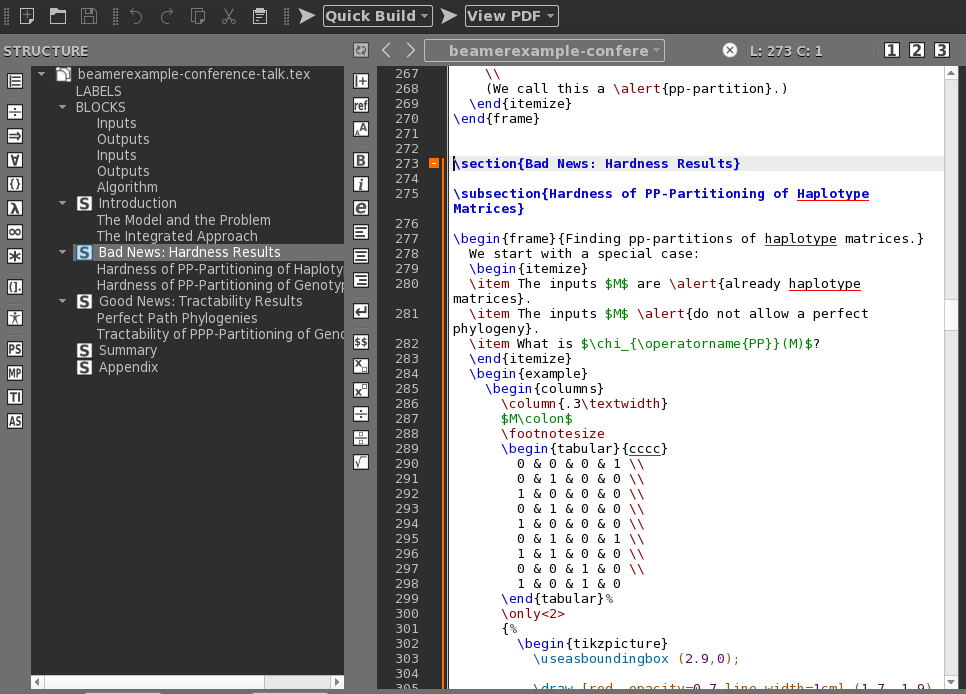
\includegraphics[width=0.99\linewidth]{../Norme_di_progetto/img/texMaker.png}
	\caption{\TeX{}maker - per la stesura dei documenti}
\end{figure}

\subsubsection{GanttProject}
GanttProject è un programma gratuito dedicato alla produzione dei diagrammi di Gantt\glo. Permette di creare task e milestone, organizzare le task in lavoro strutturato a interruzioni, disegnare
i vincoli di dipendenza tra di esse e molte altre utilità, generando automaticamente il relativo
diagramma. \\
\centerline{\url{https://www.ganttproject.biz/}}

\subsubsection{Draw.io}
Draw.io viene utilizzato per la produzione degli UML.\\
\centerline{\url{https://www.draw.io/}} 

\subsection{Gestione della configurazione}
L'obiettivo della configurazione è di creare ordine tra i documenti e il software. Tutto ciò che è configurato ha uno stato identificativo, è modificato secondo regole ben definite ed è posto sotto versionamento\glo.

\subsubsection{Versionamento}
\paragraph{Versionamento dei documenti} \mbox{} \\ \mbox{} \\
Ogni versione di qualsiasi documento deve corrispondere ad una riga della tabelle delle modifiche. il numero di versione è composto da tre cifre: \\ \\
\centerline{X.Y.Z} \\
\begin{itemize}
\item \textbf{X}: rappresenta una versione stabile del documento, resa tale dopo l'approvazione del \textit{Responsabile} di progetto: \begin{itemize}
\item inizia da 0 
\item viene incrementata di un'unità alla volta;
\end{itemize}
\item \textbf{Y}: indica l'ultima versione del documento che ha passato la fase di verifica: \begin{itemize}
\item inizia da 0;
\item viene incrementato dal verificatore ad ogni verifica;
\item quando viene incrementato X, viene riportato a 0.
\end{itemize} 
\item \textbf{Z}: indica l'ultima modifica apportata al documento dal redattore: \begin{itemize}
\item inizia da 0;
\item viene incrementato dal redattore del documento ad ogni modifica;
\item quando viene incrementato Y, viene riportato a 0.
\end{itemize}
\end{itemize}

\paragraph{GitHub} \mbox{} \\ \mbox{} \\
Per le parti del progetto da versionare si è scelto di usare GitHub\glo, un servizio del sistema di versionamento distribuito Git per contenere la repository remota. \\
I membri del team possono interagire con il VCS\glo sia da linea di comando, sia attarverso software che ne migliorano l'usabilità, come GitKraken e GitHub Desktop. La versione ufficiale del progetto è ospitata in una repository remota su GitHub, all'indirizzo \\
\centerline{\url{hhttps://github.com/teamafkSWE}}

\paragraph{Struttura del repository} \mbox{} \\ \mbox{} \\
All'interno della repository principale sopra descritta, ci sono due differenti repository: \begin{itemize}
\item \textbf{PredireConGrafana-docs}: \url{https://github.com/teamafkSWE/PredireConGrafana-docs}, contiene tutti i documenti ufficiali del progetto, suddivisi in specifiche cartelle: \begin{itemize}
\item \textbf{Cartella principale - RR}; raccoglie i file sorgenti per la compilazione dei documenti, suddivisi tra esterni ed interni, realizzati per la Revisione dei Requisiti. In futuro, saranno aggiunte cartelle distinti nominate \textbf{RP, RQ} e \textbf{RA}, contenenti i file delle rispettive consegne;
\item \textbf{Template}: contiene tutti i file che definiscono il template \LaTeX{} per la creazione di nuovi documenti;
\item \textbf{Tipologia\_di\_Documento}: ogni documento avrà la rispettiva cartella (e.i. Norme\_di\_Progetto), contenente tutti i file (sezioni ed immagini) necessari per la sua compilazione;
\end{itemize} 
\item \textbf{PredireConGrafana-SW}: \url{https://github.com/teamafkSWE/PredireConGrafana-SW}, conterrà tutti i file di codifica dei plug-in da sviluppare. 
\end{itemize}
Entrambe le repository, avranno una propria struttura identica a livello: \begin{itemize}
\item \textbf{locale}: ogni membro del gruppo lavora sui file clonati dal repositoru remoto nel proprio PC;
\item \textbf{remoto}: presente su GitHub, contiene il lavoro svolto da ogni componente e che viene condiviso con il team.
\end{itemize}


